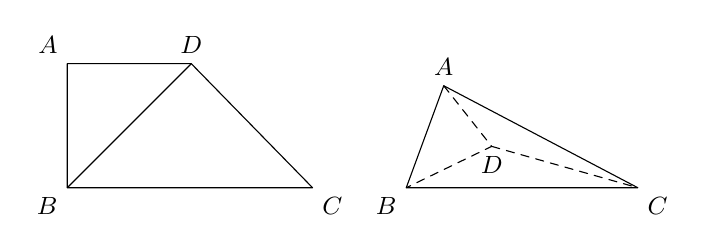
\begin{tikzpicture}[x=7mm,y=7mm,line cap=round,line join=round,every node/.style={font=\small}]
  % Original quadrilateral at left and the triangular pyramid after folding along BD at right.
  \coordinate (A1) at (0,2.25);
  \coordinate (B1) at (0,0);
  \coordinate (D1) at (2.25,2.25);
  \coordinate (C1) at (4.45,0);
  \draw (A1)--(D1)--(C1)--(B1)--cycle;
  \draw (B1)--(D1);
  \node[above left] at (A1) {$A$};
  \node[above] at (D1) {$D$};
  \node[below left] at (B1) {$B$};
  \node[below right] at (C1) {$C$};

  \coordinate (B2) at (6.15,0);
  \coordinate (C2) at (10.35,0);
  \coordinate (A2) at (6.83,1.85);
  \coordinate (D2) at (7.70,.75);
  \draw (B2)--(A2)--(C2)--(B2);
  \draw[dash pattern=on 3pt off 2.5pt] (A2)--(D2)--(B2) (D2)--(C2);
  \node[above] at (A2) {$A$};
  \node[below left] at (B2) {$B$};
  \node[below right] at (C2) {$C$};
  \node[below] at (D2) {$D$};
\end{tikzpicture}
